%% Experiments %%%%%%%%%%%%%%%%%%%%%%%%%%%%%% 

% %% Datasets %%%%%%%%%%%%%%%%%%%%%%%%%%%%%%
% \subsection{Datasets}
% \label{sec:datasets}
% %%%%%%%%%%%%%%%%%%%%%%%%%%%%%%%%%%%%%%%%%%%%%%%%%%%%%%%%%%%%


%% Experimental setup %%%%%%%%%%%%%%%%%%%%%%%%%%%%%%
\subsection{Experimental Setup}
\label{sec:experimental-setup}
%%%%%%%%%%%%%%%%%%%%%%%%%%%%%%%%%%%%%%%%%%%%%%%%%%%%%%%%%%%%

%% Evaluation Metrics %%%%%%%%%%%%%%%%%%%%%%%%%%%%%%
% \subsection{Evaluation metrics}
% \label{sec:evaluation-metrics}
%%%%%%%%%%%%%%%%%%%%%%%%%%%%%%%%%%%%%%%%%%%%%%%%%%%%%%%%%%%%
\paragraph{Evaluation metrics.} Following the evaluation metrics in \cite{gao2017tall}, we adopt two metrics (`R@$n$,IoU=$m$' and `R@$n$,mIoU').
`R@$n$,IoU=$m$' denotes the percentage of at least one of the top-$n$ predicted temporal locations having a temporal Intersection over Union (IoU) with a ground truth larger than $m$.
`R@$n$,mIoU' denotes the average of the highest IoUs among the $n$ predicted temporal locations.
% On the ActivityNet-Captions dataset, we set the predefined $n$ to 1 or 5 and $m$ to 0.1, 0.3 or 0.5.
% On the Charades-STA dataset, we set the predefined $n$ to 1 or 5 and $m$ to 0.3, 0.5 or 0.7.

\begin{table}[t!]
  \centering
  \resizebox{\columnwidth}{!}{
  \begin{tabular}{l ccc ccc}
    \toprule
    \multirow{2}{*}{Method} & \multicolumn{3}{c}{R@1,IoU=} & \multicolumn{3}{c}{R@5,IoU=} \\ 
     & 0.1 & 0.3 & 0.5 & 0.1 & 0.3 & 0.5\\
    \midrule
    Random & 38.23 & 18.64 & 7.63 & 75.74 & 52.78 & 29.49 \\
    WS-DEC & 62.71 & 41.98 & 23.34 & - & - & - \\
    MARN & - & 47.01 & 29.95 & - & 72.02 & 57.49 \\
    VCA & 67.96 & 50.45 & 31.00 & 92.14 & 71.79 & 53.83 \\
    EC-SL & 68.48 & 44.29 & 24.16 & - & - & - \\
    % BAR~\cite{wu2020reinforcement} & - & 49.03 & 30.73 & - & - & - \\
    SCN & 71.48 & 47.23 & 29.22 & 90.88 & 71.56 & 55.69 \\
    RTBPN & 73.73 & 49.77 & 29.63 & 93.89 & 79.89 & 60.56 \\
    % CTF~\cite{chen2020look} & 74.20 & 44.30 & 23.60 & - & - & - \\
    % WSLLN~\cite{gao2019wslln} & 75.40 & 42.80 & 22.70 & - & - & - \\
    LCNet & 78.58 & 48.49 & 26.33 & 93.95 & 82.51 & 62.66 \\
    CCL & - & 50.12 & 31.07 & - & 77.36 & 61.29 \\
    WSTAN & 79.78 & 52.45 & 30.01 & 93.15 & 79.38 & 63.42 \\
    FSAN & 78.45 & 55.11 & 29.43 & 92.59 & 76.79 & 63.32 \\
    CWSTG & 71.86 & 46.62 & 29.52 & 93.75 & 80.92 & 66.61 \\
    % MSCL~\cite{mo2022multi} & 75.61 & 55.05 & \textbf{38.23} & 95.26 & 82.72 & 68.05\\
    CPL & \underbar{82.55} & 55.73 & 31.37 & 87.24 & 63.05 & 43.13 \\
    \midrule
    CRM$^*$ & 81.61 & 55.26 & 32.19 & - & - & - \\
    CNM$^*$ & 78.13 & 55.68 & \underbar{33.33} & - & - & - \\
    IRON$^*$ & \textbf{84.42} & \underbar{58.95} & \textbf{36.27} & \textbf{96.74} & \textbf{85.60} & \underbar{68.52} \\
    \midrule
    PPS & 81.84 & \textbf{59.29} & 31.25 & \underbar{95.28} & \underbar{85.54} & \textbf{71.32} \\
    \bottomrule
  \end{tabular}}
  \caption{Performance comparisons on the ActivityNet Captions. The best results and second best results are represented as bold and underlined numbers, respectively. The methods using additional annotations or large-scale pre-trained models are marked with $^*$.} 
  % \\ \small{$^*$: using additional annotations or large-scale pre-trained model.}
  \label{tab:comparisons-activitynet}
\end{table}





% \begin{table}[t!]
%   \centering
%   \resizebox{\columnwidth}{!}{
%   \begin{tabular}{l ccc ccc}
%     \toprule
%     \multirow{2}{*}{Method} & \multicolumn{3}{c}{R@1} & \multicolumn{3}{c}{R@5} \\ 
%      & IoU=0.1 & IoU=0.3 & IoU=0.5 & IoU=0.1 & IoU=0.3 & IoU=0.5\\
%     \midrule
%     Random & 38.23 & 18.64 & 7.63 & 75.74 & 52.78 & 29.49 \\
%     WS-DEC & 62.71 & 41.98 & 23.34 & - & - & - \\
%     MARN & - & 47.01 & 29.95 & - & 72.02 & 57.49 \\
%     VCA & 67.96 & 50.45 & 31.00 & 92.14 & 71.79 & 53.83 \\
%     EC-SL & 68.48 & 44.29 & 24.16 & - & - & - \\
%     % BAR~\cite{wu2020reinforcement} & - & 49.03 & 30.73 & - & - & - \\
%     SCN & 71.48 & 47.23 & 29.22 & 90.88 & 71.56 & 55.69 \\
%     RTBPN & 73.73 & 49.77 & 29.63 & 93.89 & 79.89 & 60.56 \\
%     % CTF~\cite{chen2020look} & 74.20 & 44.30 & 23.60 & - & - & - \\
%     % WSLLN~\cite{gao2019wslln} & 75.40 & 42.80 & 22.70 & - & - & - \\
%     LCNet & 78.58 & 48.49 & 26.33 & 93.95 & 82.51 & 62.66 \\
%     CCL & - & 50.12 & 31.07 & - & 77.36 & 61.29 \\
%     WSTAN & 79.78 & 52.45 & 30.01 & 93.15 & 79.38 & 63.42 \\
%     FSAN & 78.45 & 55.11 & 29.43 & 92.59 & 76.79 & 63.32 \\
%     CWSTG & 71.86 & 46.62 & 29.52 & 93.75 & 80.92 & 66.61 \\
%     % MSCL~\cite{mo2022multi} & 75.61 & 55.05 & \textbf{38.23} & 95.26 & 82.72 & 68.05\\
%     CPL & \underbar{82.55} & 55.73 & 31.37 & 87.24 & 63.05 & 43.13 \\
%     \midrule
%     CRM$^*$ & 81.61 & 55.26 & 32.19 & - & - & - \\
%     CNM$^*$ & 78.13 & 55.68 & \underbar{33.33} & - & - & - \\
%     IRON$^*$ & \textbf{84.42} & \underbar{58.95} & \textbf{36.27} & \textbf{96.74} & \textbf{85.60} & \underbar{68.52} \\
%     \midrule
%     PPS & 81.84 & \textbf{59.29} & 31.25 & \underbar{95.28} & \underbar{85.54} & \textbf{71.32} \\
%     \bottomrule
%   \end{tabular}}
%   \caption{Performance comparisons on the ActivityNet Captions. The best results and second best results are represented as bold and underlined numbers, respectively. The methods using additional annotations or large-scale pre-trained models are marked with $^*$.} 
%   % \\ \small{$^*$: using additional annotations or large-scale pre-trained model.}
%   \label{tab:comparisons-activitynet}
% \end{table}




%% ActivityNet Captions Dataset %%%%%%%%%%%%%%%%%%%%%%%%%%%%%%
\paragraph{The ActivityNet Captions dataset}~\cite{krishna2017dense}
contains 37,417, 17,505, and 17,031 video-sentence pairs for training, validating $val_1$, and $val_2$, respectively.
Since a testing set is not publicly available, $val_2$ is used for testing.
Video segment features are extracted via C3D~\cite{tran2015learning}.
Vocabulary sizes are 8,000.
For proposals, $K$, $E_{en}$, and $\sigma$ are set to $5$, $2$, and $4$.
For losses, $\alpha_1$, $\alpha_2$, $\alpha_3$, and $\alpha_4$ are set to $1$, $0.2$, $0.01$, and $0.1$.

%% Charades-STA Dataset %%%%%%%%%%%%%%%%%%%%%%%%%%%%%%
\paragraph{The Charades-STA dataset}~\cite{gao2017tall}
contains 16,128 video-sentence pairs from 6,672 videos, which are divided into 12,408 for training and 3,720 for testing.
Video segment features are extracted via I3D~\cite{carreira2017quo}.
Vocabulary sizes are 1,111.
For proposals, $K$, $E_{en}$, and $\sigma$ are set to $7$, $3$, and $9$.
For losses, $\alpha_1$, $\alpha_2$, $\alpha_3$, and $\alpha_4$ are set to $3$, $5$, $0.001$, and $1$.

\paragraph{Implementation details.} We set the maximum number of video segments to 200, and the maximum length of the sentence query to 20.
For the transformers, we use transformers with three-layer and four attention heads.
The dimension of the features ($d_V$, $d_Q$, $d_G$, $d_R$) is set to 256.
We use the equivalent MC Transformer for every reconstruction process.
For the hidden sentence query, we randomly hide a third ($1/3$) of the words.
For training, the Adam optimizer~\cite{kingma2014adam} is used.
We set the learning rate to 0.0004, mini-batch size to 32, and hyper-parameters as $\lambda_1=\lambda_2=0.15$, $\beta_1=0.1$, and $\beta_2=0.15$.
In the $k^{th}$ positive proposal, we set the number of Gaussian masks $E_p$ to $k$ for reflecting a varying number of masks in each proposal, as shown in the top right of \cref{fig:framework}.
% More implementation details are described in Supplementary material.

\begin{table*}[t!]
  \centering
  \resizebox{0.95\linewidth}{!}{
  \begin{tabular}{cc c cccc}
    \toprule
    \multirow{2}{*}{Component} & \multirow{2}{*}{Strategy} & Loss & \multicolumn{2}{c}{R@1} & \multicolumn{2}{c}{R@5} \\ 
     &  & $\mathcal{L}_{pull}$ \& $\mathcal{L}^{intra}_{push}$ & IoU=0.3 & mIoU & IoU=0.3 & mIoU \\
    \midrule
    \multirow{2}{*}{Proposal type} 
     & Single Gaussian & \xmark & 47.49 & 33.33 & 78.23 & 54.85 \\
     & Gaussian mixture & \cmark & \textbf{59.29} & \textbf{37.59} & \textbf{85.54} & \textbf{58.78} \\
    \midrule
    \multirow{3}{*}{Gaussian generation} 
     & Learning one center \& multiple widths & \xmark & 46.63 & 31.54 & 83.65 & \textbf{59.49} \\
     & Learning multiple centers \& widths & \cmark & 47.82 & 32.08 & 84.09 & 56.35 \\ 
     & Learning multiple centers \& one width  & \cmark & \textbf{59.29} & \textbf{37.59} & \textbf{85.54} & 58.78 \\
     \midrule
     \multirow{3}{*}{Importance weighting} & No importance & \cmark & 52.55 & 34.56 & 79.67 & 58.41 \\
     & Importance from the generator & \cmark & 48.55 & 32.36 & 78.96 & 56.87 \\ 
     & Importance from the reconstructor & \cmark & \textbf{59.29} & \textbf{37.59} & \textbf{85.54} & \textbf{58.78} \\ 
    \bottomrule
  \end{tabular}
  }
  \caption{Ablation studies of Gaussian mixture proposals on the ActivityNet Captions dataset.}

  \label{tab:ablation-positive-proposals}
\end{table*}

 
\begin{table}[t!]
  \centering
  \resizebox{\columnwidth}{!}{
  \begin{tabular}{l ccc ccc}
    \toprule
    \multirow{2}{*}{Method} & \multicolumn{3}{c}{R@1,IoU=} & \multicolumn{3}{c}{R@5,IoU=} \\ 
     & 0.3 & 0.5 & 0.7 & 0.3 & 0.5 & 0.7\\
    \midrule
    Random & 20.12 & 8.61 & 3.39 & 68.42 & 37.57 & 14.98 \\
    TGA & 32.14 & 19.94 & 8.84 & 86.58 & 65.52 & 33.51 \\
    % CTF~\cite{chen2020look} & 39.80 & 27.30 & 12.90 & -  & - & - \\
    SCN & 42.96 & 23.58 & 9.97 & 95.56 & 71.80 & 38.87 \\
    WSTAN & 43.39 & 29.35 & 12.28 & 93.04 & 76.13 & 41.53 \\
    % BAR~\cite{wu2020reinforcement} & 44.97 & 27.04 & 12.23 & -  & - & - \\
    VLANet & 45.24 & 31.83 & 14.17 & 95.70 & 82.85 & 33.09 \\
    MARN & 48.55 & 31.94 & 14.81 & 90.70 & 70.00 & 37.40 \\
    % WSRA~\cite{fang2020weak} & 50.13 & 31.20 & 11.01 & 86.75 & 70.50 & 39.02 \\
    CCL & - & 33.21 & 15.68 & - & 73.50 & 41.87 \\
    RTBPN & 60.04 & 32.36 & 13.24 & 97.48 & 71.85 & 41.18 \\
    LoGAN & 51.67 & 34.68 & 14.54 & 92.74 & 74.30 & 39.11 \\
    VCA & 58.58 & 38.13 & 19.57 & 98.08 & 78.75 & 37.75 \\
    LCNet & 59.60 & 39.19 & 18.87 & 94.78 & 80.56 & 45.24 \\
    CWSTG & 43.31 & 31.02 & 16.53 & 95.54 & 77.53 & 41.91 \\
    % MSCL~\cite{mo2022multi} & 58.92 & 43.15 & 23.49 & 98.02 & 81.23 & 48.45 \\
    CPL & 66.40 & 49.24 &
    22.39 & 96.99 & 84.71 & 52.37 \\
    \midrule
    CRM$^*$ & 53.66 & 34.76 & 16.37 & -  & - & - \\
    CNM$^*$ & 60.39 & 35.43 & 15.45 & -  & - & - \\
    IRON$^*$ & \textbf{70.71} & \textbf{51.84} & \underbar{25.01} & \underbar{98.96} & \textbf{86.80} & \textbf{54.99} \\
    \midrule
    PPS & \underbar{69.06} & \underbar{51.49} & \textbf{26.16} & \textbf{99.18} & \underbar{86.23} & \underbar{53.01} \\
    \bottomrule
  \end{tabular}}
  \caption{Performance comparisons on the Charades-STA.
  The best results and second best results are represented as bold and underlined numbers, respectively. The methods using additional annotations or large-scale pre-trained models are marked with $^*$.} 
  % \\ \small{$^*$: using additional annotations or large-scale pre-trained model.}
  \label{tab:comparisons-charades}
\end{table}




% \begin{figure}[t!]
%   \centering
%     \begin{subfigure}[b]{\linewidth}
%          \centering
%          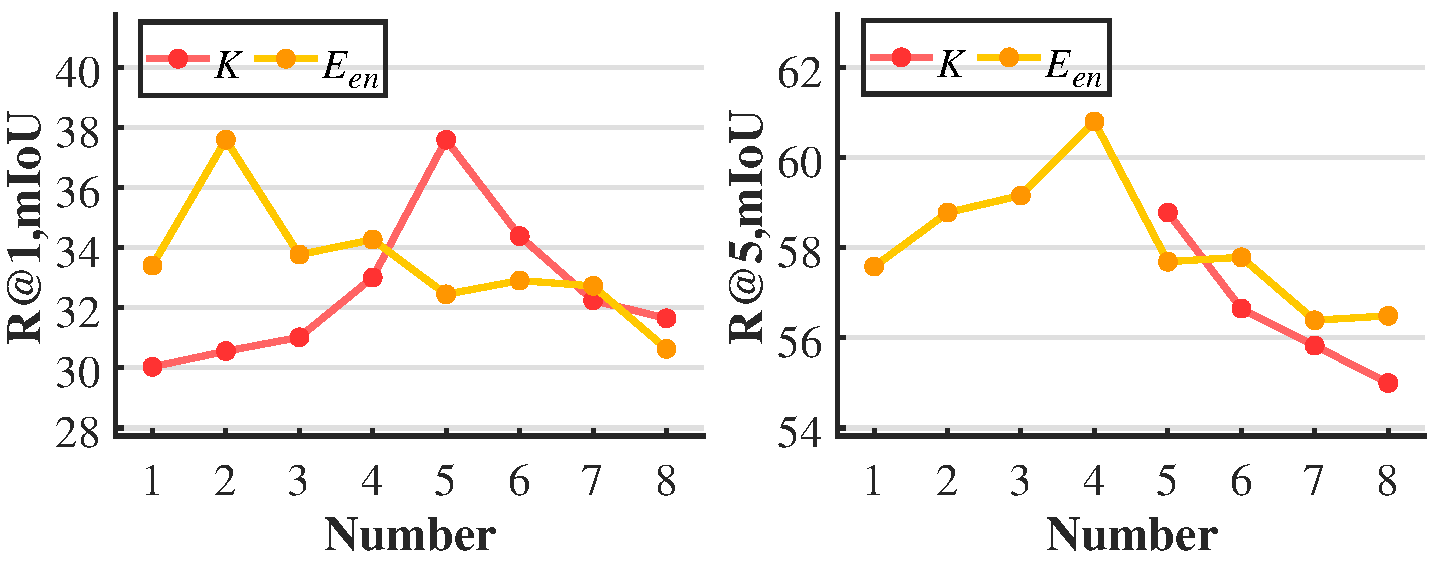
\includegraphics[width=\linewidth]{figures/3-ablation-graph-props.pdf}
%          \caption{}
%          \label{fig:ablation-graph-props}
%     \end{subfigure}
%     \vfill
%     \begin{subfigure}[b]{\linewidth}
%          \centering
%          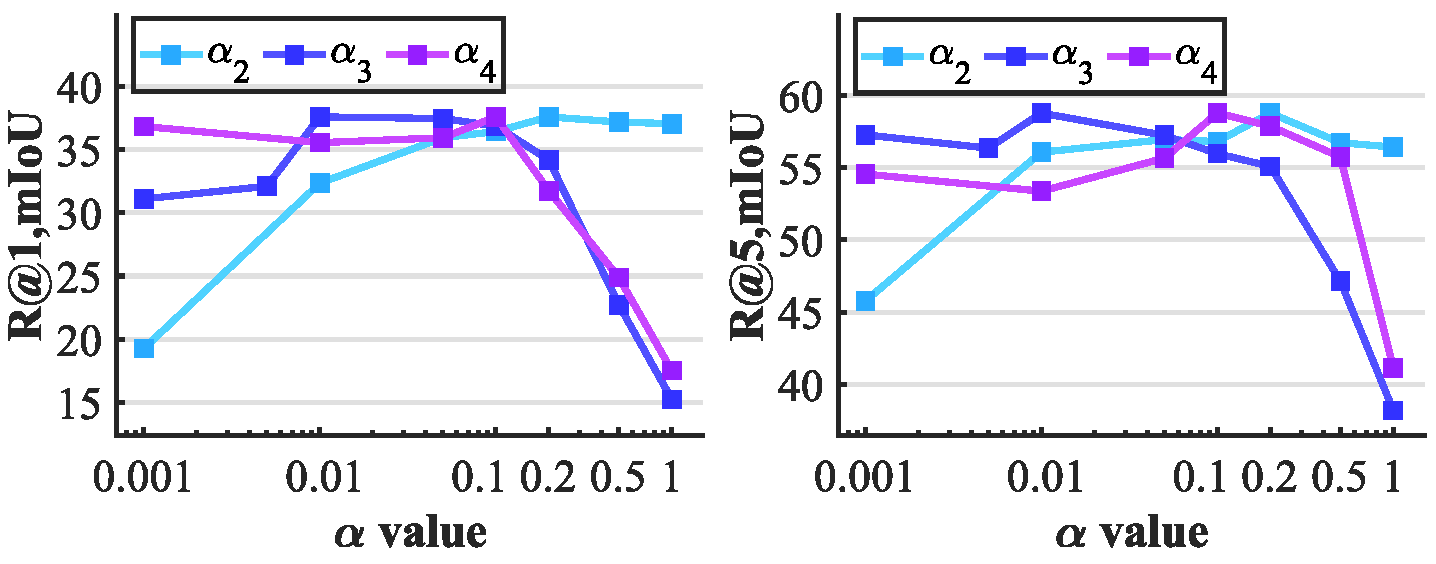
\includegraphics[width=\linewidth]{figures/3-ablation-graph-alpha.pdf}
%          \caption{}
%          \label{fig:ablation-graph-alpha}
%     \end{subfigure}
%     \caption{Ablation studies by varying (a) the number of proposals $K$ and the number of negative masks $E_{en}$ for each easy negative proposal and (b) $\alpha$ values for the pull-push learning scheme on the ActivityNet Captions dataset.
%     % $\alpha$, $\alpha_3$, and $\alpha_4$ for balancing losses
%     }
% \label{fig:ablation-graph}
% \end{figure}

%% Comparison with State-of-the-Arts %%%%%%%%%%%%%%%%%%%%%%%%%%%%%%
\subsection{Comparison with State-of-the-Art Methods}
\label{sec:comparison-with-state-of-the-art-methods}
%%%%%%%%%%%%%%%%%%%%%%%%%%%%%%%%%%%%%%%%%%%%%%%%%%%%%%%%%%%%
To verify the effectiveness of the proposed method, we compare our PPS with previous weakly supervised temporal video grounding methods:
WS-DEC~\cite{duan2018weakly},
TGA~\cite{mithun2019weakly},
SCN~\cite{lin2020weakly},
WSTAN~\cite{wang2021weakly},
VLANet~\cite{ma2020vlanet},
MARN~\cite{song2020weakly},
CCL~\cite{zhang2020counterfactual},
RTBPN~\cite{zhang2020regularized},
EC-SL~\cite{chen2021towards},
LoGAN~\cite{tan2021logan},
VCA~\cite{wang2021visual},
LCNet~\cite{yang2021local},
FSAN~\cite{wang2022fine},
CWSTG~\cite{Chen_Luo_Zhang_Ma_2022},
CPL~\cite{zheng2022cpl},
CRM~\cite{huang2021cross},
CNM~\cite{zheng2022cnm}, and
IRON~\cite{cao2023iterative}.

In \cref{tab:comparisons-activitynet} for the ActivityNet Captions dataset, our PPS outperforms CPL~\cite{zheng2022cpl} by $3.56\%$, $22.49\%$, and $28.19\%$ at R@1,IoU=0.3, R@5,IoU=0.3, and R@5,IoU=0.5, respectively.
It is worth noting that PPS outperforms the previous learnable mask-based method, CPL, by significant margins at R@5, which means that the generated proposals of PPS promise a higher level of quality.
In \cref{tab:comparisons-charades} for the Charades-STA dataset, our PPS surpasses CPL~\cite{zheng2022cpl} by $3.77\%$ and $2.19\%$ at R@1,IoU=0.7 and R@5,IoU=0.3, respectively.
The methods marked with $^*$ make unfair comparisons with the previous methods.
CRM~\cite{huang2021cross} uses additional paragraph description annotations. CNM~\cite{zheng2022cnm} uses CLIP large-scale pre-trained features~\cite{radford2021learning} and IRON~\cite{cao2023iterative} uses OATrans~\cite{wang2022object} and DistilBERT~\cite{sanh2019distilbert} large-scale pre-trained features.
Although our PPS uses 3D ConvNet and Glove features for fair comparisons with previous methods, PPS shows competitive or higher performance with the methods marked with $^*$.
% To study the impact of large-scale pre-trained features, we conduct the experiment using CLIP features in Supplementary material.

\begin{figure}[t!]
  \centering
  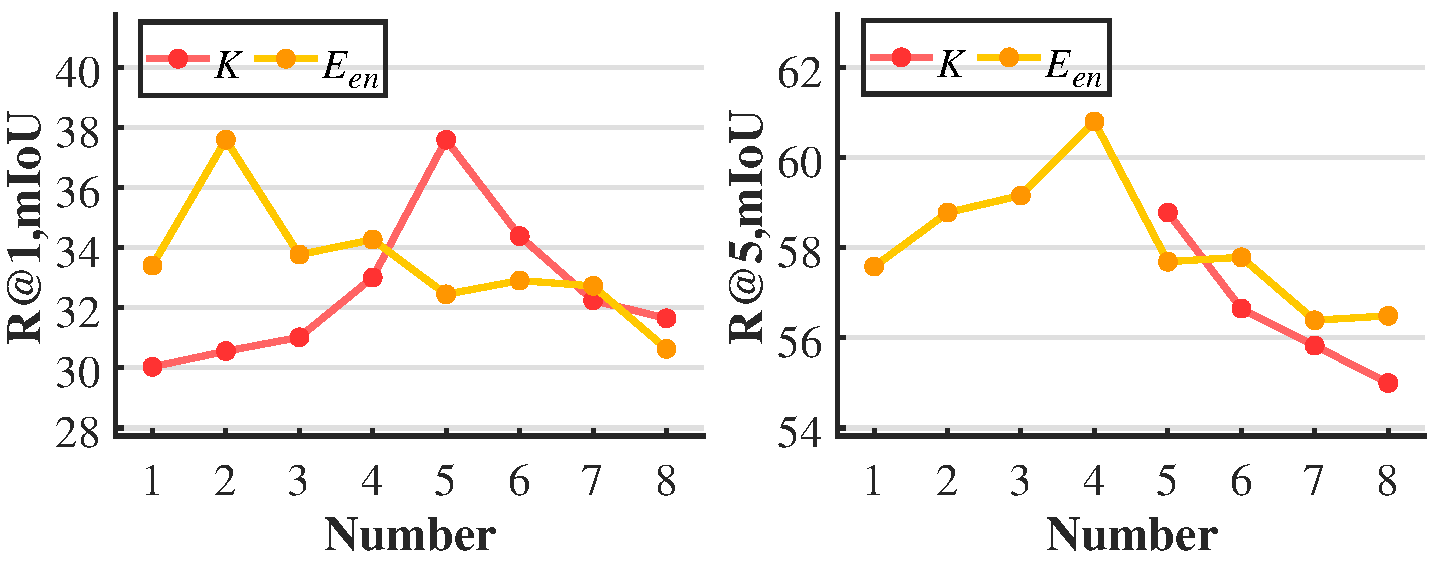
\includegraphics[width=\linewidth]{figures/3-ablation-graph-props.pdf}
    \caption{Ablation studies by varying the number of positive and negative proposals $K$ and the number of Gaussian masks of an easy negative proposal $E_{en}$.
    }
    \label{fig:ablation-graph-props}
\end{figure}

%% Ablation Study %%%%%%%%%%%%%%%%%%%%%%%%%%%%%%
\subsection{Ablation Study}
\label{sec:ablation-study}
%%%%%%%%%%%%%%%%%%%%%%%%%%%%%%%%%%%%%%%%%%%%%%%%%%%%%%%%%%%%
For a more in-depth understanding of the proposed method, we perform ablation studies on our components.
% More details of the variants used in the ablation studies are explained in Supplementary material.

\paragraph{Analysis on the Gaussian mixture proposal.}
As shown in \cref{tab:ablation-positive-proposals}, we study the impact of the different strategies to generate Gaussian mixture proposals for positive proposals.
The results are summarized as follows:
First, the Gaussian mixture proposals are more effective than the single Gaussian proposal, which means that the mixture proposal can better represent a query-relevant temporal location.
Second, learning multiple centers and one width for one mixture proposal performs best.
We conjecture that learning multiple widths makes it complicated to learn proposals, which reduces performance.
Third, importance weighting from the reconstructor yields the best result by representing the importance of each mask for query reconstruction.
On the other hand, importance weighting from the generator is less effective, because it is hard to reflect reconstruction-aware information.
\cref{fig:ablation-graph-props} shows the impact of the number of proposals $K$.
The performance increases until the number is $5$ at R@1,mIoU.
We observe that defining too many proposals makes the proposals redundant and have short lengths due to the impact of the inter-pushing loss $\mathcal{L}^{inter}_{push}$.


\paragraph{Impact on a varying number of masks.}
For positive proposals, we form $\mathbf{P}_{p}^{(k)}$ by a Gaussian mixture of $E_p=k$ Gaussian masks to reflect a varying number of Gaussian masks in each positive proposal.
To verify the effectiveness of the varying number of Gaussian masks, we compare the performance of fixing the number of Gaussian masks for every positive proposal in \cref{tab:ablation-positive-proposals-fixing}.
The results show that using a varying number of Gaussian masks for each positive proposal performs better than using a fixed Gaussian number of Gaussian masks.
We find that combinations of different numbers of Gaussian masks can represent a diverse number of query-relevant events.

\begin{table}[t!]
  \centering
          \begin{subtable}[t]{.47\linewidth}
            \centering
              \resizebox{\columnwidth}{!}{
              \begin{tabular}{c cc}
                \toprule
                \multirow{2}{*}{\# masks} & R@1 & R@5 \\ 
                 & mIoU & mIoU \\
                \midrule
                Fix to 1 & 33.33 & 54.85 \\ 
                Fix to 3 & 35.91 & 56.27 \\ 
                Fix to 5 & 36.58 & 54.36 \\ 
                Fix to 7 & 36.25 & 49.48 \\ 
                \midrule
                Vary & \textbf{37.59} & \textbf{58.78} \\ 
                \bottomrule
          \end{tabular}}
        \caption{The number of masks for a positive proposal.}
          \label{tab:ablation-positive-proposals-fixing}
            \end{subtable}%
        \hspace{0.2cm}
        \begin{subtable}[t]{.47\linewidth}
                  \centering
                      \resizebox{\columnwidth}{!}{
                      \begin{tabular}{c cc}
                        \toprule
                        Pulling & R@1 & R@5 \\ 
                        strategy & mIoU & mIoU \\
                        \midrule
                        All & 35.41 & 56.87 \\ 
                        To mid & 35.83 & \textbf{58.92} \\ 
                        Distant & \textbf{37.59} & 58.78 \\ 
                        \bottomrule
                \end{tabular}}
                \caption{Strategies for the pulling loss}
              \label{tab:ablation-pulling-loss}
        \end{subtable}%
        \caption{Ablation studies on the ActivityNet Captions dataset.}
    % \hspace{0.5cm}
  %   \begin{subtable}[t]{.335\linewidth}
  %       \centering
  %             \caption{Ablation studies of hard \& easy negative proposals.}
  %             \resizebox{\columnwidth}{!}{
  %             \begin{tabular}{cc cc}
  %               \toprule
  %               \multirow{2}{*}{Negative proposal} & \multirow{2}{*}{$\mathcal{L}_{ivc}$} & R@1 & R@5 \\ 
  %                &  & mIoU & mIoU \\
  %               \midrule
  %               None & \xmark & 31.44 & 53.08 \\ 
  %               Only hard & \cmark & 32.49 & 56.23 \\ 
  %               Only easy & \cmark & 30.75 & 57.21 \\ 
  %               Both hard \& easy & \cmark & \textbf{37.59} & \textbf{58.78} \\ 
  %               \bottomrule
  %         \end{tabular}}
  %         \label{tab:ablation-negative-proposal-loss}
          
  % \end{subtable}
  \label{tab:ablation-others}
\end{table}



% \begin{table*}[t!]
%   \centering
%   \caption{Ablation studies on different strategies of PPS on the ActivityNet Captions dataset.}
%           \begin{subtable}[t]{.275\linewidth}
%             \centering
%               \caption{Performance comparisons by fixing the number of masks.}
%               \resizebox{\columnwidth}{!}{
%               \begin{tabular}{c cc}
%                 \toprule
%                 \multirow{2}{*}{Positive proposal} & R@1 & R@5 \\ 
%                  & mIoU & mIoU \\
%                 \midrule
%                 Varying num & \textbf{37.59} & \textbf{58.78} \\ \midrule
%                 Fixing to 1 & 33.33 & 54.85 \\ 
%                 Fixing to 3 & 35.91 & 56.27 \\ 
%                 Fixing to 5 & 36.58 & 54.36 \\ 
%                 Fixing to 7 & 36.25 & 49.48 \\ 
%                 \bottomrule
%           \end{tabular}}
%           \label{tab:ablation-positive-proposals-fixing}
%             \end{subtable}%
%         \hspace{0.5cm}
%         \begin{subtable}[t]{.31\linewidth}
%                   \centering
%                       \caption{Performance comparisons by varying strategies for the pulling loss $\mathcal{L}_{pull}$.}
%                       \resizebox{\columnwidth}{!}{
%                       \begin{tabular}{c cc}
%                         \toprule
%                         \multirow{2}{*}{$\mathcal{L}_{pull}$ strategy} & R@1 & R@5 \\ 
%                         & mIoU & mIoU \\
%                         \midrule
%                         Pulling all masks & 35.41 & 56.87 \\ 
%                         Pulling to the mid & 35.83 & \textbf{58.92} \\ 
%                         Pulling distant masks & \textbf{37.59} & 58.78 \\ 
%                         \bottomrule
%                 \end{tabular}}
%               \label{tab:ablation-pulling-loss}
%         \end{subtable}%
%     \hspace{0.5cm}
%   %   \begin{subtable}[t]{.335\linewidth}
%   %       \centering
%   %             \caption{Ablation studies of hard \& easy negative proposals.}
%   %             \resizebox{\columnwidth}{!}{
%   %             \begin{tabular}{cc cc}
%   %               \toprule
%   %               \multirow{2}{*}{Negative proposal} & \multirow{2}{*}{$\mathcal{L}_{ivc}$} & R@1 & R@5 \\ 
%   %                &  & mIoU & mIoU \\
%   %               \midrule
%   %               None & \xmark & 31.44 & 53.08 \\ 
%   %               Only hard & \cmark & 32.49 & 56.23 \\ 
%   %               Only easy & \cmark & 30.75 & 57.21 \\ 
%   %               Both hard \& easy & \cmark & \textbf{37.59} & \textbf{58.78} \\ 
%   %               \bottomrule
%   %         \end{tabular}}
%   %         \label{tab:ablation-negative-proposal-loss}
          
%   % \end{subtable}
%   \label{tab:ablation-others}
% \end{table*}



  
\begin{table}[t!]
  \centering
  \resizebox{\columnwidth}{!}{
  \begin{tabular}{ccc cccc}
    \toprule
    \multicolumn{3}{c}{Loss} & \multicolumn{2}{c}{R@1,IoU=} & \multicolumn{2}{c}{R@5,IoU=} \\ 
    $\mathcal{L}_{pull}$ & $\mathcal{L}^{intra}_{push}$ & $\mathcal{L}^{inter}_{push}$ & 0.3 & mIoU & 0.3 & mIoU \\
    \midrule
    \xmark & \xmark & \xmark & 45.23 & 30.98 & 67.86 & 47.75 \\
    \cmark & \xmark & \xmark & 55.03 & 36.79 & 72.49 & 51.14 \\
    \xmark & \cmark & \xmark & 45.69 & 29.83 & 71.51 & 49.69 \\
    \xmark & \xmark & \cmark & 23.50 & 15.96 & 72.30 & 44.46 \\
    \xmark & \cmark & \cmark & 23.47 & 16.38 & 66.15 & 38.20 \\
    \cmark & \xmark & \cmark & 41.51 & 30.23 & 85.18 & \textbf{60.44} \\
    \cmark & \cmark & \xmark & 49.98 & 32.46 & 80.54 & 55.26 \\ 
    \cmark & \cmark & \cmark & \textbf{59.29} & \textbf{37.59} & \textbf{85.54} & 58.78 \\ 
    \bottomrule
  \end{tabular}}
  \caption{Ablation studies of different losses for the pull-push learning scheme on the ActivityNet Captions dataset.}
  \label{tab:ablation-loss}
\end{table}



\paragraph{Effect of the pull-push learning scheme.}
In \cref{tab:ablation-loss}, we verify the effectiveness of our pull-push learning scheme.
Among combinations of three losses ($\mathcal{L}_{pull}$, $\mathcal{L}^{intra}_{push}$, $\mathcal{L}^{inter}_{push}$), adopting all three losses yields the best performance.
We conjecture that our pull-push learning scheme helps Gaussian masks to capture diverse events for better representing a temporal location.
It is notable that adopting only the pulling loss can yield competitive or higher results to the state-of-the-art methods in \cref{tab:comparisons-activitynet}.
If the pulling loss $\mathcal{L}_{pull}$ is excluded, the performance decreases significantly.
We observe that Gaussian masks for one Gaussian mixture proposal are spread sparsely throughout the entire video without $\mathcal{L}_{pull}$, which can not represent one proper temporal location.
Additionally, the results suggest that two pushing losses ($\mathcal{L}^{intra}_{push}$, $\mathcal{L}^{inter}_{push}$) are used with $\mathcal{L}_{pull}$ for a synergy effect, because the goal of the pushing losses is to make less overlapped masks for moderate coupling.
For a more in-depth understanding of the pulling loss $\mathcal{L}_{pull}$, we conduct ablation studies of different strategies for $\mathcal{L}_{pull}$ in \cref{tab:ablation-pulling-loss}.
Among the strategies, pulling two distant masks closer or pulling two distant masks to the middle mask performs best.
The results imply that pulling fewer masks is better and pulling more masks may ruin the structure of the mixture proposal due to overlapped masks.
\cref{fig:ablation-graph-alpha} presents the impact of controlling the balance of the losses.
The results show that a high $\alpha_2$ value for $\mathcal{L}_{pull}$ is needed to produce densely generated masks and the adequate $\alpha_3$ and $\alpha_4$ values for $\mathcal{L}^{intra}_{push}$ and $\mathcal{L}^{inter}_{push}$ are needed to cause proper discrimination between the masks and between the proposals, respectively.

\begin{figure}[t!]
  \centering
    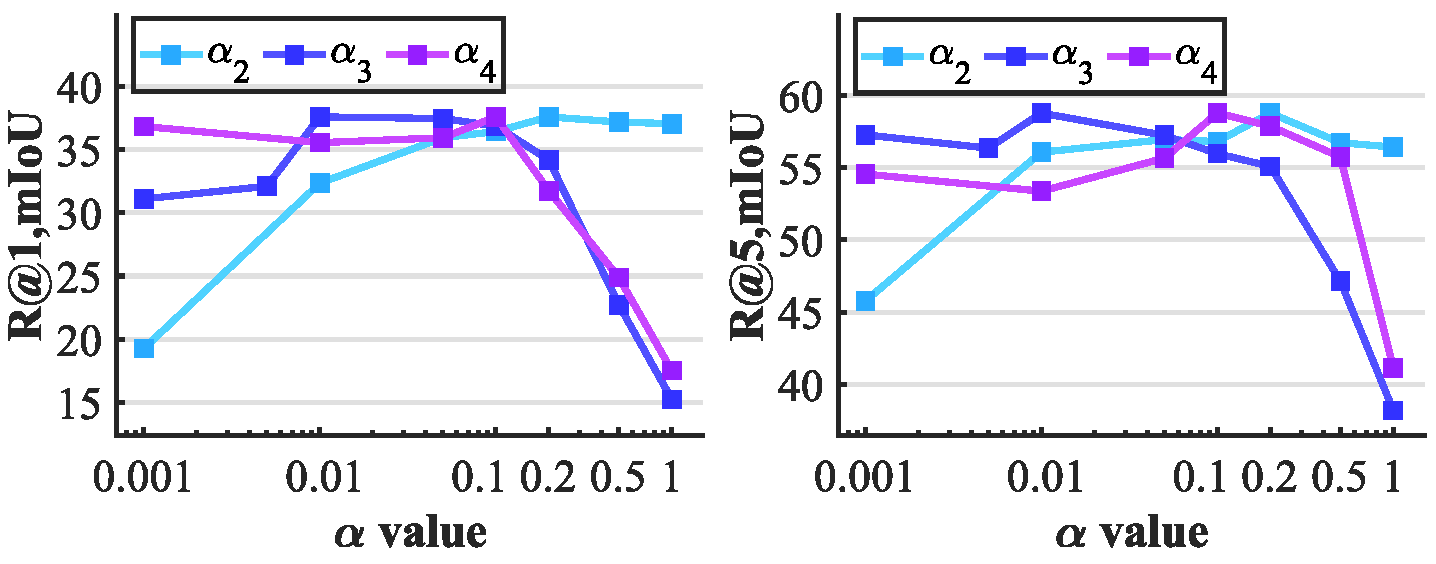
\includegraphics[width=\linewidth]{figures/3-ablation-graph-alpha.pdf}
    \caption{Ablation studies by varying $\alpha$ values for the pull-push learning scheme on the ActivityNet Captions dataset.
    }
    \label{fig:ablation-graph-alpha}
\end{figure}

%% Qualitative Results %%%%%%%%%%%%%%%%%%%%%%%%%%%%%%
\subsection{Qualitative Results}
\label{sec:qualitative-results}
%%%%%%%%%%%%%%%%%%%%%%%%%%%%%%%%%%%%%%%%%%%%%%%%%%%%%%%%%%%%

\cref{fig:qualitative} shows qualitative results of our PPS and other variants of PPS.
It is notable that PPS captures accurate query-relevant locations, while the ground truth, which can be noisy due to the subjectivity of annotators, includes redundant locations such as a logo at the beginning of the video.
% More qualitative results for the visualization of proposals are shown in Supplementary material.


\begin{figure}[t]
  \centering
  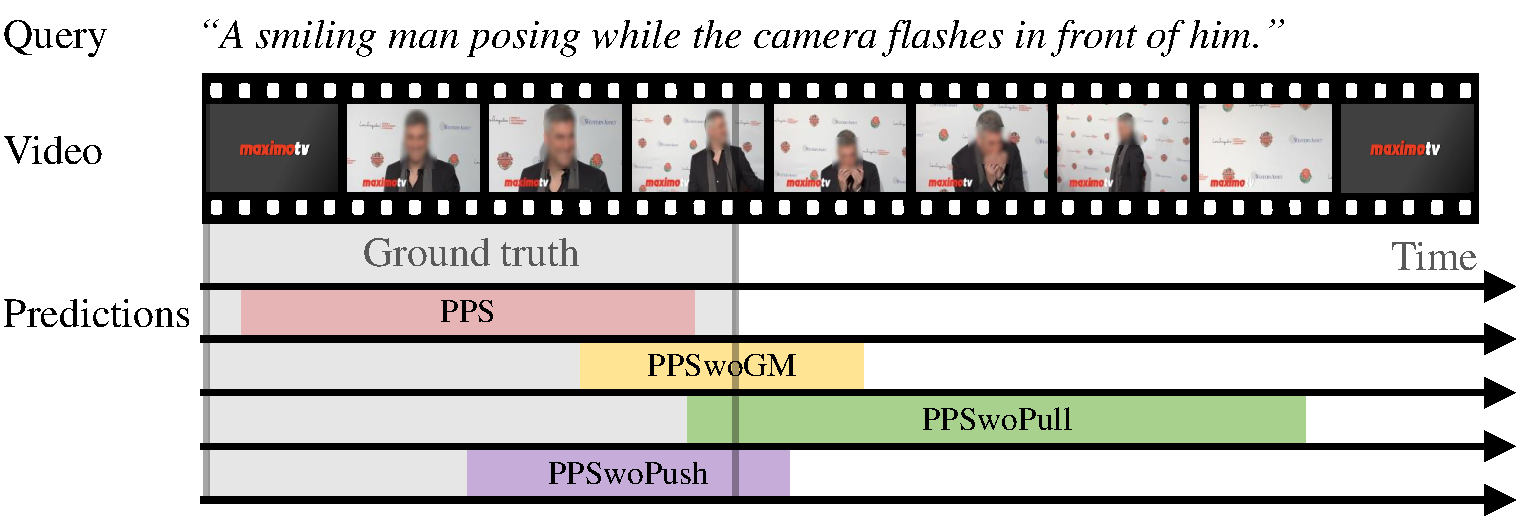
\includegraphics[width=\linewidth]{figures/4-qualitative.pdf}
  \caption{
  Qualitative results on the Activity-Net Captions dataset.
  Given a video and a query, PPS yields a predicted temporal location (red).
  We also visualize the predictions of variants using a positive proposal of one Gaussian mask without the mixture (yellow) or excluding a pulling loss (green) or excluding pushing losses (purple).
  }
\label{fig:qualitative}
\end{figure}